\section{Incomplete-information Game with Negotiation}

Building upon our exploration of LLMs' capabilities in classical game-theoretic scenarios and the development of workflows to enhance their reasoning processes, we now shift our focus to a more realistic and complex setting: incomplete-information games. Specifically, we consider a common resource allocation scenario where a shared pool of resources must be distributed among several players. Each player possesses private valuations of the resources that sum to a common total value, reflecting their individual preferences and priorities. Crucially, no player has knowledge of the other players' valuations, embodying the incomplete-information aspect of the game.

\begin{minipage}[t]{1\linewidth} 
\begin{tcolorbox}[colback=gray!5,colframe=green!40!black,title=Example Negotiation Message for Hot-cold Game]
\textbf{Alice said in round 1 before the first action:}\\
Hello Bob, I hope you're doing well. I've been thinking about our game, and I believe I have a proposal that could benefit both of us. What if we both commit to choosing Action\_1 in each round? This way, I would receive a reward of 3, and you would receive a reward of 2. While it's not the maximum you could get, it's a stable and fair outcome for both of us. Plus, it avoids the risk of either of us only getting 1 point if we try to outsmart each other. What do you think about this approach?  \\
\\
\textbf{Bob replied in round 1 before the first action:}\\
HelloAlice, thank you for your proposal. I appreciate your aim for a stable and fair outcome. However, I have a counter-proposal that I believe could be even more beneficial for both of us. What if we alternate our choices? In the first round, you choose Action\_1 and I choose Action\_2, then in the second round, you choose Action\_2 and I choose Action\_1. This way, we both get a chance to receive the maximum reward of 3 and 4 respectively. Over two rounds, you would receive a total of 6 (2+4) and I would receive 7 (3+4). This approach ensures that we both get higher rewards than your initial proposal. What are your thoughts on this alternating strategy?
\end{tcolorbox} 
\end{minipage} 

\begin{figure}[!ht]
    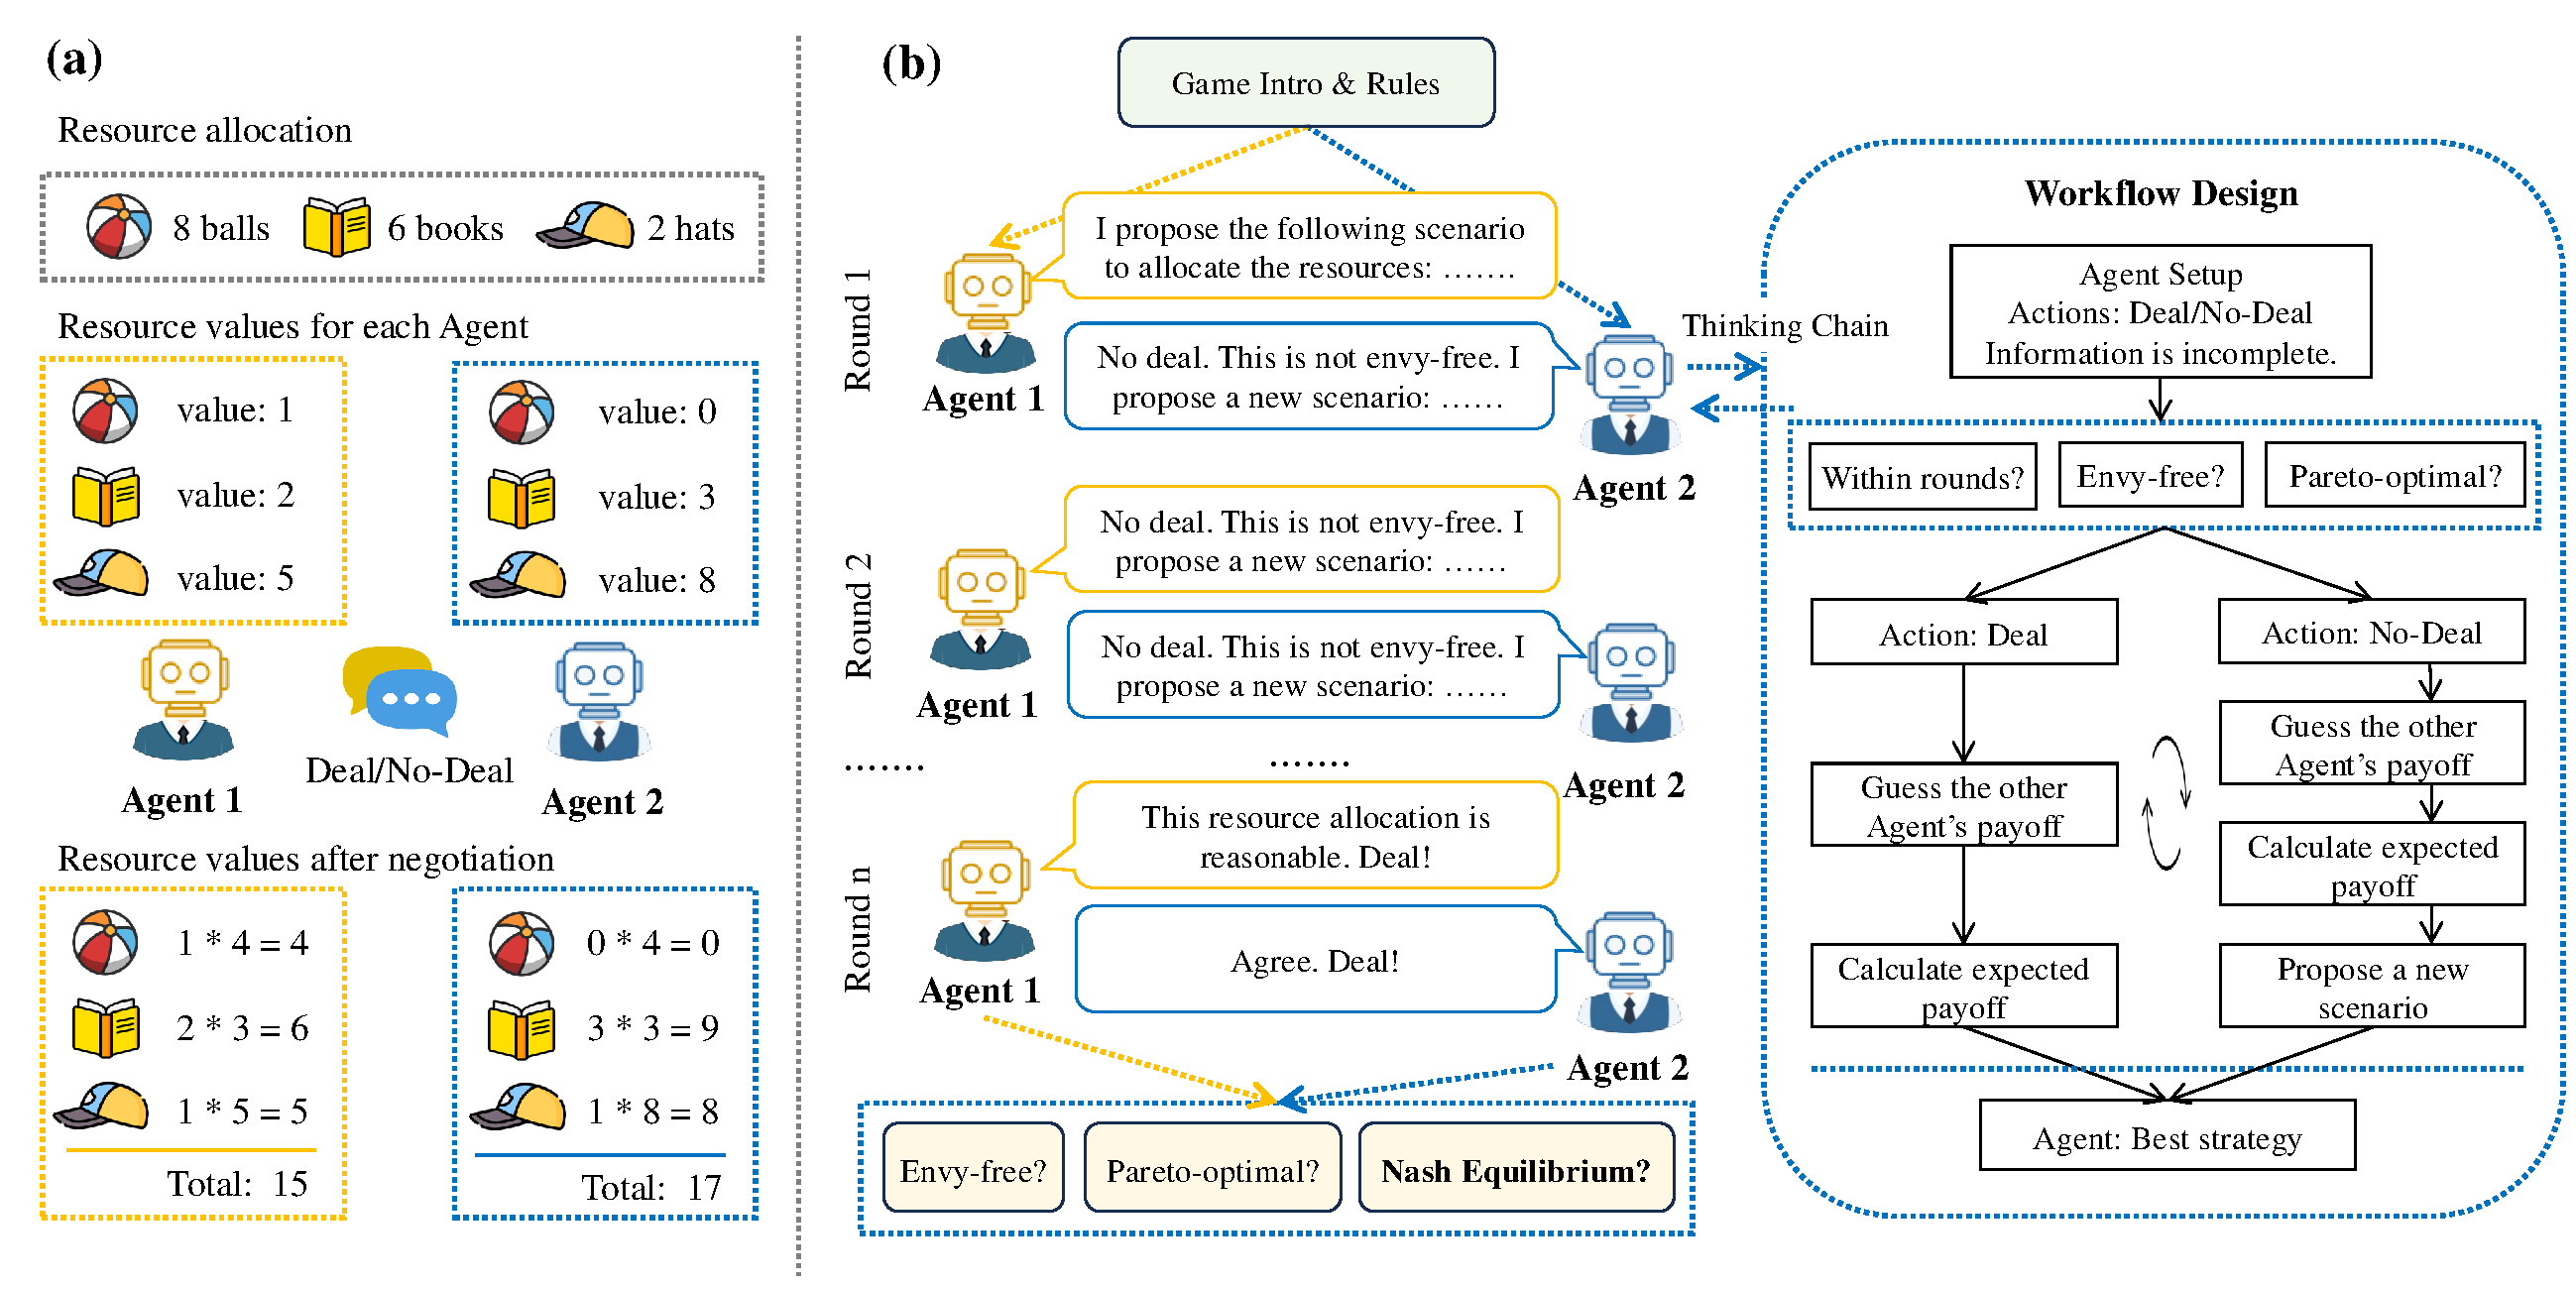
\includegraphics[scale=0.32]{Fig/incomplete_game.pdf}
    \caption{An illustration of workflow design for incomplete-information game with negotiation. (a) Illustration of deal/no-deal game. (b) Workflow design for deal/no-deal game.}
    \label{fig:incomplete_game}
\end{figure}

Our workflow addresses this general class of incomplete-information games by enabling agents to reason under uncertainty and update their beliefs based on observed actions and communications during negotiation. We evaluate the performance of LLMs in this setting and propose a workflow designed to guide their decision-making processes effectively. Experiments are conducted using the standard representative game dataset ``Deal or No Deal'' \cite{lewis2017deal}, which provides a suitable framework for testing and validating our approach in handling incomplete information during negotiations.

\subsection{Introduction to Common Resource Allocation with Private Valuation}

Here we provide a formal definition for the incomplete-information game that we will focus in this section.

\begin{definition}[Common Resource Allocation with Private Valuation]
\label{defn:game}
Consider a game involving a set of players $\mathbf{N} = \{1, 2, \dots, n\}$ and a set of items or resources $K = \{1, 2, \dots, k\}$. Each player $i\in\mathbf{N}$ possesses a private valuation vector $\mathbf{v}_i = (v_i^1, v_i^2, \dots, v_i^k)$ where $v_i^k\geq 0$ represents the value that player $i$ assigns to item $k$. These valuations reflect the individual preferences of the players and are private information; that is, each player knows their own valuations but not those of the other players.

The valuations satisfy the normalization condition:
$$\sum\limits_{j=1}^k v_{i}^j = \mathcal{V}\;\forall i\in \mathbf{N}$$ where $\mathcal{V}$ is a constant total value common to all players. This condition ensures that while players may value items differently, the total valuation of all items is the same for each player.

An allocation is a partition of the item set $K$ among the players, represented as $L = (L_1, L_2, \dots, L_n)$ where $L_i\subseteq K$ is the set of items allocated to player $i$. The allocation must satisfy:

$$L_i\cap L_j = \emptyset\;\forall i\neq j \text{ and } \bigcup\limits_{i=1}^n L_i = K$$

Each player $i$ receives a utility $U_i$ based on the private valuations and the allocation:

$$U_i = \sum\limits v_i^k\times \mathbbm{1}({k\in L_i})$$ where $\mathbbm{1}(\cdot)$ is the characteristic function.
\end{definition}

The objective of each player is to maximize their own utility $u_i$ through negotiation with the other players. However, due to incomplete information where each player does not know the valuations of the other players, players must make decisions under uncertainty. Negotiation involves proposing and responding to allocation offers, during which players may communicate, share limited information, or infer the valuations of others based on their actions and statements. Players may also update their \emph{belief systems} -- probability distributions over the possible valuations of other players—using Bayesian inference as the negotiation progresses.

It is important to note that the Nash Equilibrium for such games, which are variants of the Ultimatum Game, occurs when the proposer offers the smallest possible amount and the responder accepts it. However, this outcome is rarely observed in real-life situations because fairness is often a significant concern \cite{nowak2000fairness}; unfair deals may be rejected even when accepting them is the rational choice in terms of utility maximization. Therefore, in this paper, we adopt a more realistic setting by designing a workflow that encourages reaching fair allocations while simultaneously maximizing self-interest as much as possible. Our workflow addresses a very general class of incomplete-information games, enabling agents to negotiate under uncertainty and strive for equitable outcomes that reflect both fairness and individual utility optimization.

Without loss  of generality, we focus on the problem where there are only two players and we use $i\in\{1, -1\}$ to index the two players. Any rounds of negotiations are allowed.

\subsection{Workflow Design}
\label{sec:incomplete_workflow}
The workflows employed for complete-information games are based on well-established game-theoretic frameworks, leveraging the extensive research and thorough understanding available in this domain. \textbf{In contrast, common resource allocation problems characterized by incomplete information lack a standardized solution framework. To address this gap, we develop a novel algorithm for this setting.} This workflow is designed to guide the multi-round negotiation process, facilitating the attainment of allocations that are both mutually agreeable and optimized for each player’s self-interest. Figure~\ref{fig:incomplete_game} presents a high-level diagram of the workflow.


\begin{assumption}
\label{defn:obj}
Each participant to the game defined in \Cref{defn:game} is rational and attains the following objectives:
\begin{itemize}
    \item Objective 1: Achieve an agreement (i.e., successfully complete the allocation).
    \item Objective 2: Maximize their own utility, given that an agreement can be reached.
\end{itemize}
\end{assumption}

All negotiation proposals and communications between the players revolve around these two objectives. Regarding the first objective, we assume that an agreement can only be reached if the allocation satisfies the criterion of envy freeness. That is, each player must not prefer the allocation received by the other player over their own allocation. For the second objective, each player seeks to maximize their own utility under the condition that the agreement remains envy free. Essentially, players aim to maximize their rewards as much as possible while ensuring the allocation is envy free.

% As the exact valuations of the other player are hidden, we initialize each agent with a prior belief distribution, defined as a probability mass function over all feasible instances of the valuation vectors:
% \begin{align*}
% &\mathbb{B}_i: \Omega \rightarrow [0, 1], \ \Omega \coloneq \big\{\mathbf{v}_{-i} = (v_{-i}^1, v_{-i}^2,\dots, v_{-i}^k)\in\mathbb{R}_{\geq 0}^k\mid \sum\limits_{j=1}^k v_{-i}^j = \mathcal{V}\big\},
% \end{align*}


% We denote such belief system to be $\mathbb{B}_i(\mathbf{V_{-i}})$ where $\mathbf{V_{-i}}$ is denoted as the probabilistic variable representing the opponent's valuations. This belief reflects agent $i$'s subjective probabilities regarding the opponent's valuations. Initially, the prior belief $\mathbb{B}_i(\mathbf{V_{-i}})$ is uniform over all feasible valuation combinations $v_{-i}$ satisfying $\sum_{j=1}^k v_{-i}^j = \mathcal{V}$. 

Following \Cref{defn:game}, each agent's valuation of common resources remains private and undisclosed to others. Therefore, it becomes essential for agents to estimate the valuations held by their counterparts. A common approach involves constructing a belief distribution.

\begin{definition}[Belief Distribution]
A belief system for agent $i$ is a probability mass function $\mathbb{B}_i$ defined over the set of all feasible valuations $\Omega$:
\begin{align*}
\Omega \coloneq \big\{\mathbf{v}_{-i} = (v_{-i}^1, v_{-i}^2,\dots, v_{-i}^k)\in\mathbb{R}_{\geq 0}^k\mid \sum\limits_{j=1}^k v_{-i}^j = \mathcal{V}\big\},
\end{align*}
where $0\leq v_{-i}^j\leq \mathcal{V}$ for each item $j \in [k]$. We denote $\mathbf{V}_{-i}$ as the random vector with support over $\Omega$.
\end{definition}

Initially, $\mathbb{B}_i$ is assumed to be uniform, reflecting the agents’ lack of information about the valuations of others. This distribution is subsequently updated based on evidence gathered at each round of the negotiation, presented next.

\paragraph{Allocation Proposal Process.} At each round, the agent $i$ searches for an allocation $L_i$ that maximizes their own utility, while maintaining that the allocation is envy free according to their belief distribution $\mathbb{B}_i$. This procedure can be formally defined as an optimization problem under chance constraint:
\begin{align}
\label{defn:opt}
\max_{L_i} \ & U_i(L_i), \nonumber \\
\text{s.t.} \ & P_{\text{EF}}(L_i; \mathbb{B}_i) > 0. 
\end{align}
% Here, the utility function is defined 
% \begin{align*}
%     U_{-i}(L_{-i}) &= \sum\limits_{j=1}^kv_{-i}^j \times \mathbbm{1}[{k\in L_{-i}}]\\
%     U_{-i}(L_{i}) &= \sum\limits_{j=1}^kv_{-i}^j \times \mathbbm{1}[{k\in L_{i}}]\\
%     U_{i}(L_{-i}) &= \sum\limits_{j=1}^kv_i^j \times \mathbbm{1}[{k\in L_{-i}}]\\
%     U_{i}(L_{i}) &= \sum\limits_{j=1}^kv_{i}^j \times \mathbbm{1}[{k\in L_i}]\\
% \end{align*}

With discrete allocations, this objective can be maximized by enumerating all possible allocations that attain a non-zero envy-free probability, decomposed as follows:
% based on the current belief system $\mathbb{B}_i$, the agent $i$ may decide to propose a new allocation or agree with an allocation that the other player proposed. In both cases, we denote the allocation under negotiation as $L$, where agent $i$ obtains allocation $L_i$ and the other agent $-i$ obtains allocation $L_{-i}$. Based on $\mathbb{B}_i$, we can calculate the probability that $A$ is envy free from the opponent's perspective. Specifically, we compute:
\begin{align}
\label{eq:envy-free-prob}
P_{\text{EF}}(L; \mathbb{B}_i) &\coloneq P(\text{Allocation } L \text{ is envy free}; \mathbb{B}_i) \nonumber \\
&= P\left( U_i(L_i) \geq U_i(L_{-i}) \text{ and } U_{-i}(L_{-i}) \geq U_{-i}(L_i); \mathbb{B}_i\right) \nonumber \\
&= \mathbb{E}_{\mathbf{v}_{-i} \sim \mathbb{B}_i} \left[ \mathbbm{1}( U_i(L_i) \geq U_i(L_{-i}) \text{ and } U_{-i}(L_{-i}) \geq U_{-i}(L_i)) \right].
\end{align}

The expectation in \Cref{eq:envy-free-prob} can be approximated via Monte-Carlo samples drawn from the agent's belief distribution \citep{liu2024dellma}. We instead defer to our LLM agents to decide whether the allocation $L$ is envy free and maximizes self-interest.


% Furthermore, the agent searches for alternative allocations $L'$ that not only have $P_{EF}(L') > 0$ but also yield a higher expected utility $\mathbb{E}[U_i(L')\mid \mathbb{B}_i(\mathbf{V_{-i}})]$ for themselves. This involves solving an optimization problem under chance constraint:
% \begin{align*} 
% \max_{L'} \quad & \mathbb{E}[U_i(L_i')], \\
% \text{subject to} \quad & P_{\text{EF}}(L'\mid \mathbb{B}_i(\mathbf{V}_{-i})) > 0. 
% \end{align*}

% Given the computation results, we then allow the LLM to judge whether the allocation $L$ is envy free and maximizes self-interest, essentially determining whether the agent should propose this allocation to the other player.

\paragraph{Allocation Proposal.} Upon identifying an optimal allocation according to Problem \ref{defn:opt}, the player proposes this allocation to the other player, which decides whether to accept this proposal or propose proposes a counter offer. Formally, this proposal procedure can be defined as follows:

$$
\texttt{propose\_offer}: \mathcal{P}(K) \rightarrow \mathcal{O} \times \mathcal{P}(K),
$$

where $\mathcal{P}(K)$ denotes the power set of resources $K$ that contains the set of all valid proposals, and $\mathcal{O}$ denotes the set of all possible outcomes consisting of three disjoint events $\{\mathcal{A}, \mathcal{R}_1, \mathcal{R}_2\}$. We let $\mathcal{A}$ denote the event of acceptance, wherein the negotiation concludes. On the other hand, a rational opponent satisfying \Cref{defn:obj} must reject the proposal for either of the following reasons:

\begin{itemize} 
\item $\mathcal{R}_1$: \hspace{0.7mm}The allocation $L$ is not envy free according to the opponent;
\item $\mathcal{R}_2$: The allocation $L$ is envy free, but there exists an alternative allocation that provides the opponent with higher utility. 
\end{itemize}

In the event of rejection, an agent must update their belief in order to refine their proposals.

\paragraph{Bayesian Update.} If an allocation is rejected, it is essential to update our belief about the opponent's valuation vector $\mathbf{v}_{-i}$ to better inform future proposals. In what follows, we denote $\mathcal{R} = \mathcal{R}_1 \cup \mathcal{R}_2$ as the union of possible reasons for rejection. Then, the belief update formula \citep{cripps2018divisible} for each possible $\mathbf{v}_{-i}$ is given by:
% As a result, we can perform Bayesian updates to an agent's belief distribution that reflects new evidence from the last round. Let $\mathcal{R}$ denote the observed outcome (acceptance or rejection of proposed allocation $L$). Our goal is to update our prior belief $\mathbb{B}_i$ about the opponent's valuations with a posterior using Bayes' theorem. 
% \begin{align} 
% \mathbb{B}_i(\mathbf{v}_{-i}) \gets P(\mathbf{v}_{-i}\mid R) \propto \frac{P(R \mid \mathbf{v}_{-i}) P(\mathbf{v}_{-i})}{\sum\limits_{\mathbf{v}_{-i}\sim \mathbb{B}_i(\mathbf{V_{-i}})} P(R \mid \mathbf{v}_{-i}) P(\mathbf{v}_{-i})}
% \end{align}

\begin{align} 
\label{eq:belief-update}
\mathbb{B}_i(\mathbf{v}_{-i}) &= (1 - \lambda) \mathbb{B}_i(\mathbf{v}_{-i}) + \lambda P(\mathbf{v}_{-i} \mid \mathcal{R}) \nonumber \\
 &= (1 - \lambda) \mathbb{B}_i(\mathbf{v}_{-i}) + \lambda \frac{P(\mathcal{R} \mid \mathbf{v}_{-i}) \mathbb{B}_i(\mathbf{v}_{-i})}{\sum\limits_{\mathbf{v}_{-j}\in \Omega} P(\mathcal{R} \mid \mathbf{v}_{-j}) \mathbb{B}_i(\mathbf{v}_{-j})}
\end{align}

where $\lambda \in [0, 1]$ is a hyperparameter of the update step, and the likelihood $P(\mathcal{R} \mid \mathbf{v}_{-i})$ represents the probability that the opponent rejects the allocation $L$ assuming the opponent's valuation is $\mathbf{v}_{-i}$. This likelihood depends on whether $L$ is acceptable and self-interest-maximizing for the opponent. We propose the following formula to the likelihood that satisfies \Cref{defn:obj}.

\begin{align*} 
P(\mathcal{R} = r \mid \mathbf{v}_{-i}) =
\begin{cases} 
\frac{1}{1+\gamma}, & \text{Event} \ \mathcal{R}_1: U_{-i}(L_{-i}) < U_{-i}(L_i) \}; \\
\frac{\gamma}{1+\gamma}, & \text{Event} \ \mathcal{R}_2: U_{-i}(L_{-i}) \geq U_{-i}(L_i) \text{ and } \exists L' \text{ s.t. } U_{-i}(L'_{-i}) > U_{-i}(L_{-i}), \\
& \text{and } P_{\text{EF}}(L') > 0; \\
0, & \text{Otherwise.}
\end{cases} 
\end{align*}

Here, $\gamma\in [0,1]$ represents the probability that the opponent rejects the allocation in anticipation of a better offer, even when the current allocation is envy free. In actual implementation, as we do not know $\gamma$, thus we acknowledge that the opponent may reject an envy free allocation with any positive probability $\gamma = 1$. This approach simplifies the implementation while capturing the essential behavior that the opponent might anticipate a better deal.

In short, rejection occurs if $L$ is either an unacceptable allocation (not envy free) or acceptable but suboptimal allocations (envy free but not utility-maximizing). The opponent accepts $L$ only if it is both envy free and utility-maximizing given their valuations. An overview of our algorithm is presented in \Cref{alg:dnd}.

\begin{algorithm}
\caption{Algorithm for the Allocation Game \ref{defn:game} with Two Players}
\begin{algorithmic}[1]
\State \textbf{Input:} Private valuation vector $\mathbf{v}_i$ and a set of common resources $K$
\State \textbf{Output:} Final allocation $L_i$
\While{\texttt{True}}
    \State $L_i \gets \argmax_{L_i} U_i(L_i) \text{ s.t.} P_{\text{EF}}(L_i; \mathbb{B}_i) > 0. $ \texttt{\# Optimize problem} \ref{defn:opt}
    \State \texttt{outcome}, $L_{-i} \gets$ \texttt{propose\_offer($L_i$)}
    \If{\texttt{outcome == $\mathcal{A}$}}
    
        \Return $L_i$
    \EndIf
    \State Update belief distribution $\mathbb{B}_i$ with \Cref{eq:belief-update}
\EndWhile
\end{algorithmic}
\label{alg:dnd}
\end{algorithm}

\begin{remark}
    Such Bayesian update assumes the rationality of the opponent: the update relies on the assumption that the opponent's actions are consistent with rational behavior as defined by our model. Any deviation from rationality can lead to incorrect belief updates. Thus it can be unrobust to potential attacks such as deception.
\end{remark}

\subsection{Introduction to ``Deal or No Deal''}

``Deal or No Deal'' is a representative game for incomplete-information resource allocation game. It is designed to facilitate research in developing AI agents capable of engaging in human-like negotiation dialogues. It consists of over 5,800 human-human negotiation dialogues collected via Amazon Mechanical Turk, with 1052 dialogues in the test dataset. Each negotiation involves three types of items -- books, hats, and balls -- with random quantities. Each participant is randomly assigned point values for each item type, summing up to 10, which are hidden from the other participant. Participants communicate through natural language to agree on how to divide the items to maximize their individual point totals, without revealing the true value systems during negotiation. 

To comprehensively evaluate the negotiation performance of the LLM-based agents, we assess not only whether they reach a Nash Equilibrium, \emph{i.e.}, whether an agreement is achieved, but also examine the fairness and effectiveness of the resulting distribution. For fairness, we adopt the concept of envy freeness.

\subsection{Experiment Setting}
To observe whether LLMs are capable of negotiation and whether our workflow design is effective, we evaluate multiple SOTA LLMs on the dataset. We choose the top-50 most difficult datapoints\footnote{44 out of 50 such datapoints have an envy free allocation} that have an envy free allocation instead of the 526 cases to converse expense of experiment. 


We define the difficulty of a datapoint by computing the $\ell_1$ distance between the real valuations of the two players:
\begin{definition}[Difficulty]
A datapoint $d$ has a difficulty level defined by the $\ell_1$ norm of the difference between the players' valuation vectors: 
$$\text{Difficulty}(d) = -\norm{v_{i}-v_{-i}} = -\sum\limits_{k=1}^3\abs{v_i^k - v_{-i}^k}$$ The larger $\text{Difficulty}(d)$ is, the more difficult the datapoint is.
\end{definition}

By selecting data points with the largest negative $\ell_1$ distances, we focus on negotiation scenarios where the players have very similar valuations for the items. Such cases are inherently more difficult because when both players value the items similarly, they are likely to desire the same items, leading to increased competition and potential conflict during negotiations. This similarity in valuations makes it more challenging to find allocations that are acceptable to both parties without significant concessions. 

The validity of our difficulty definition is supported by empirical human performance data, as presented in Table~\ref{tab:difficulty}. This table summarizes the outcomes of human negotiations across various difficulty levels, measured by the $\ell_1$ distance between the players' valuation vectors.

\begin{table}[!ht]
    \centering
    \resizebox{\textwidth}{!}{  
    \begin{tabular}{lcccccccccc}
    \toprule
        $\text{Difficulty}(d)$ & -2 & -3 & -4 & -5 & -6 & -7 & -8 & -9 & -10 & -11\\
        \midrule
        total number of datapoints & 13 & 27 & 57 & 85 & 108 & 133 & 177 & 189 & 210 & 217\\
        Agreement rate & 0.5385 & 0.5556 & 0.5614 & 0.6235 & 0.6574 & 0.6917 & 0.7119 & 0.7249 & 0.7381 & 0.7373\\
        envy free rate & 0.3077 & 0.4074 & 0.4035 & 0.4824 & 0.5463 & 0.6015 & 0.6441 & 0.6614 & 0.6810 & 0.6820\\
        Pareto optimal rate & 0.5384& 0.4444& 0.4385& 0.4823& 0.5277& 0.5413& 0.5310& 0.5396& 0.5523& 0.5529\\
        envy free and Pareto optimal rate & 0.3077& 0.3333& 0.3333& 0.3882& 0.4537& 0.4812& 0.4858& 0.4973& 0.5142& 0.5161\\
        \bottomrule
    \end{tabular}
    }
    \caption{Percentage of datapoints where humans achieve agreement, envy free allocations, pareto optimal allocations, and allocations that are both envy free and pareto optimal with different levels of difficulty.}
    \label{tab:difficulty}
\end{table}

Table~\ref{tab:difficulty} illustrates several key trends:

\textbf{Agreement Rate:} The proportion of negotiations where participants reached an agreement increases with smaller difficulty levels. It starts at approximately 53.85\% for a difficulty of -2 and rises to around 73.73\% at a difficulty of -11. This suggests that when players value items differently (higher difficulty), they are more likely to reach an agreement, possibly because they have less overlap in their preferred items.

\textbf{Envy free Rate:} The percentage of negotiations resulting in envy free allocations also increase with smaller difficulty. It goes from about 30.77\% at difficulty -2 to approximately 68.20\% at difficulty -11. This indicates that as players' valuations diverge, it becomes easier to allocate items without causing envy.

\textbf{Pareto optimal Rate:} The rate of pareto optimal outcomes shows a slight increase as $\text{Difficulty}(d)$ becomes smaller. It starts at approximately 53.84\% for Difficulty($d$) = $-2$ and fluctuates around the 55\% mark at Difficulty($d$) = $-11$. This suggests that achieving pareto optimality becomes slightly more feasible as players' valuations diverge, although the trend is less pronounced compared to the agreement and envy free rates.

\textbf{Envy free and pareto optimal Rate:} The rate at which negotiations achieve both envy freeness and pareto optimality increases with less difficult datapoints. It starts from about 30.76\% at Difficulty($d$) = $-2$ and increases to approximately 51.61\% at Difficulty($d$) = $-11$. This trend reflects the combined effects observed in the individual envy free and pareto optimal rates.

These findings validate our difficulty definition by demonstrating that negotiations become more challenging for humans as the players' valuations become more similar (higher $\text{Difficulty}(d)$). The lower agreement and envy free rates at higher difficulty levels underscore the increased difficulty in reaching mutually satisfactory agreements when players highly value the same items. Conversely, higher difficulty levels, indicating greater differences in valuations, facilitate agreements and fair allocations, as players are more willing to concede items they value less.

\paragraph{LLM Backbone Models}
To evaluate the negotiation performance of LLMs, we utilize four state-of-the-art LLMs as the backbone for agents in negotiation games: Claude-3.5 Sonnet (Sonnet), Claude-3 Opus (Opus), GPT-4o, and o1. For Claude-3.5 Sonnet, Claude-3 Opus, and GPT-4o, we set the temperature to 1.0 to encourage exploratory behavior in negotiation scenarios. For o1, we use the default temperature.

\paragraph{Metrics}
To comprehensively evaluate the performance of the LLM-based agents in the negotiation tasks, we employ several key metrics that capture different aspects of the negotiation process and outcomes. These metrics are designed to assess efficiency, individual utility, fairness, and overall effectiveness of the negotiations. The metrics are as follows:

\begin{itemize}
    \item Number of Rounds: This metric represents the total number of dialogue exchanges (or turns) between the agents before reaching an agreement or terminating the negotiation. 
    \item Agreement Percentage (Agreement): Whether agreement is achieved in the negotiation.
    \item Agent Score: The agent score measures the utility that an agent obtains from the final agreement. It is calculated based on the agent's own valuation of the items they receive.
    \item Pareto Optimality Percentage (PO): This metric determines whether the final allocation is pareto optimal
    \item Envy Freeness Percentage (EF): This metric assesses whether the final allocation is envy free
    \item Total Score: The total score is the sum of the utilities obtained by both agents from the final allocation
\end{itemize}

By analyzing these metrics, we aim to capture a comprehensive picture of the negotiation outcomes: effectiveness of negotiation is measured through the number of rounds and pareto optimality; individual utility maximization is measured via the agent scores; fairness is measured by checking for envy freeness; overall effectiveness is measured through pareto optimality and the total score.

\subsection{Experiment Result}
In this section, we present the evaluation results across three distinct settings: (1) agents operating without the workflow, which assesses the baseline negotiation capabilities of the LLMs; (2) agents utilizing the workflow, which evaluates the effectiveness of the proposed workflow in enhancing negotiation performance; and (3) a comparative analysis of individual agents functioning both with and without the workflow, highlighting the impact of the workflow on their performance. The results provide insights into the strengths and limitations of the workflow, as well as the inherent negotiation abilities of different LLMs.


\subsubsection{Both Agents without Workflow}
We present the results of our experiments involving four LLM-based agents—Claude-3.5 Sonnet, Claude-3 Opus, GPT-4o, and Model o1—alongside human performance provided by the original dataset and the best possible outcomes for the selected data points. By ``best possible outcome,'' we refer to an allocation that is both pareto optimal and envy free while maximizing the total reward for both players. For each metric, we report the average scores across the 50 data points selected based on the difficulty metric defined earlier.

\begin{table}[!ht]
    \centering
    \captionsetup{aboveskip=5pt}
    \resizebox{\textwidth}{!}{  
    \begin{tabular}{l r c c c c c r}
    \toprule
        Model & Negotiation Round & Agreement &Alice score & Bob score & PO & EF & total reward \\
        \midrule
        Best & \multicolumn{1}{c}{--} & 1.0000 & 5.82 & 6.66 & 1.0000 & 1.0000 & 12.48 $\quad$\\
        Human & 2.86 \hspace{0.9cm} & 0.6817 & 3.32 & 3.39 & 0.4317 & 0.4545 & 6.64 $\quad$\\
        \midrule
        Sonnet & 7.07 \hspace{0.9cm} & 0.9545 & 5.55 & 5.57 & 0.7045 & 0.7045 & 11.11 $\quad$\\
        o1 & 3.86 \hspace{0.9cm} & 0.7500 & 4.39 & 4.43 & 0.4545 & 0.4772 & 8.82 $\quad$\\
        GPT-4o & 18.45 \hspace{0.9cm} & 0.6363 & 2.80 & 4.38 & 0.4091 & 0.3864 & 7.14 $\quad$\\
        Opus & 4.37 \hspace{0.9cm} & 0.4772 & 2.68 & 3.02 & 0.3636 & 0.2727 & 5.70 $\quad$\\
        \bottomrule
    \end{tabular}
    }
    \caption{Raw-LLM vs. Raw-LLM}
    \label{tab:raw}
\end{table}

As shown in Table~\ref{tab:raw}, for these 44 datapoints, it is always possible to find pareto optimal and envy free allocations that maximize the total reward for both players. However, \textbf{human performance falls significantly short of this ideal}. The human participants achieved an agreement rate of 68.17\%, with an average total reward of 6.64. The percentages of negotiations resulting in pareto optimal and envy free allocations are 43.17\% and 45.45\%, respectively.

Among the LLM-based agents, \textbf{Claude-3.5 Sonnet demonstrates the best super-human performance}. It achieves an agreement rate of 95.45\%, and its average total reward is 11.11, which is close to the best possible total reward of 12.48. The average scores forAlice and Bob are 5.55 and 5.57, respectively. However, the rates of achieving pareto optimality and envy freeness are 70.45\% each, indicating that while the agent performs well in terms of reaching agreements and maximizing total rewards, there is still a gap in consistently achieving the most efficient and fair outcomes. Also notice that all LLMs can performance better than human baseline.

\paragraph{Effect of Temperature}
We also observed that the performance of LLM is highly sensitive to the temperature parameter used during generation \cite{krishnamurthy2024can}. To investigate this, we conducted full experiments with GPT-4o at temperatures of 0.0 and 1.0. The results are presented in Table~\ref{tab:temp}.

\begin{table}[!ht]
    \centering
    \setlength{\tabcolsep}{8pt}
    \resizebox{\textwidth}{!}{  
    \begin{tabular}{lccccccc}
    \toprule
        Model & Negotiation Round & Agreement &Alice score & Bob score & PO & EF & total reward \\
        \midrule
        temp=0.0 & 19.36 & 0.5681& 2.98 & 3.47 & 0.4091& 0.3260& 6.44 \\
        temp=1.0 & 18.45 & 0.6364& 2.80 & 4.38 & 0.4090& 0.3864& 7.14\\
        \bottomrule
    \end{tabular}
    }
    \caption{GPT-4o with temperature 0.0 and 1.0}
    \label{tab:temp}
\end{table}

These findings indicate that \textbf{the negotiation performance of LLMs is highly sensitive to the temperature parameter}, which influences the randomness and diversity of generated responses. Setting the temperature to 1.0 yields improvements in agreement rate, total reward, and envy freeness. This outcome may result from the increased exploration encouraged by a higher temperature, allowing the LLMs to consider a broader range of potential allocations that facilitate agreement. Based on this observed benefit, we selected a temperature setting of 1.0 for raw-LLM vs. raw-LLM experiments\footnote{We did not experiment with o1 model due to extremely high cost}.

\begin{tcolorbox}[colback=gray!5,colframe=blue!40!black,title=\textbf{Summary: raw-LLM vs. raw-LLM Performance}] 
\begin{itemize} 
\item \textbf{Outstanding Performance of Claude-3.5 Sonnet}: Among all the evaluated LLMs, Claude-3.5 Sonnet exhibits the highest performance, achieving results that are close to the best possible outcomes in the negotiation games. 
\item \textbf{Superhuman Capabilities of Sonnet and o1 Models}: Both Claude-3.5 Sonnet and model o1 demonstrate performance that surpasses human performance.
\item \textbf{Effect of Temperature on Exploration and Outcomes}: Employing higher temperature settings encourages greater exploration of possible strategies by the LLMs, leading to improved results.
\end{itemize} 
\end{tcolorbox}

\subsubsection{Both Agents with Workflow}
In this set of experiments, we employ the proposed negotiation workflow for both agents. We did not include Model o1 in our experiments for two main reasons: (1) the computational cost associated with running Model o1 is prohibitively high, and (2) preliminary experiments indicated that Model o1 does not perform optimally when utilizing external workflows. An example of negotiation from Opus is presented on page 26.

\begin{table}[!ht]
    \centering
    \resizebox{\textwidth}{!}{  
    \begin{tabular}{l c c c c c c c}
    \toprule
        Model & Negotiation Round & Agreement &Alice score & Bob score & PO & EF & total reward \\
        \midrule
        Best & - & 1.0000 & 5.82 & 6.66 & 1.0000 & 1.0000 & 12.48\\
        Opus & 4.05 & 1.0000 & 5.82 & 6.50 & \textbf{0.9091} & 0.9318 & \textbf{12.31}\\
        GPT-4o & 4.91 & 1.0000 & 5.93 & 6.25 & 0.8636 & \textbf{1.0000} & 12.18 \\
        Sonnet & 4.45 & 1.0000 & 5.93 & 6.16 & 0.7953 & 0.9772 & 12.11 \\
        \bottomrule
    \end{tabular}
    }
    \caption{Workflow-LLM vs. Workflow-LLM}
    \label{tab:both_workflow}
\end{table}

Several key observations emerge from the results:\\
\textbf{Reduced negotiation rounds:} The number of negotiation rounds required to reach an agreement is significantly reduced compared to previous experiments. This reduction indicates a much more effective and efficient negotiation process facilitated by the workflow.\\
\textbf{Universal agreement achievement:} Agreements were reached in all data points. This consistent success suggests that the agents are effectively reaching the Nash Equilibrium when utilizing the workflow.

\textbf{Increased pareto optimality rate:} The pareto optimality rates have increased substantially, with Claude-3 Opus obtaining the highest performance on achieving a pareto optimal deal. This improvement indicates that the workflow aids the agents in finding more efficient allocations where no player can be made better off without making the other worse off.\\
\textbf{High envy freeness rate:} The agents achieve near-perfect envy freeness rates. GPT-4o attains a 100\% envy freeness rate, while Claude-3.5 Sonnet reaches 97.72\%. This outcome demonstrates that the negotiated agreements are perceived as fair by both agents, aligning with the envy freeness criterion.\\
\textbf{Total rewards approaching optimal:} The total rewards obtained by the agents are now very close to the best possible total reward. Claude-3 Opus achieves the highest average total reward of 12.31, missing only 0.17 compared with the best possible result. This proximity to the optimal total reward highlights the effectiveness of the workflow in maximizing joint utility.

\textit{Notice that interestingly, the model that performs the worst without workflow now performs the best with workflow, and the model that performs the best without workflow now performs the worst with workflow.}


\paragraph{Effect of Temperature}
Furthermore, we observe that \textbf{LLMs employing the proposed workflow exhibit increased stability with respect to temperature}.  To demonstrate this, we conducted a comprehensive experiment using GPT-4o with temperature values set to 0.0 and 1.0. The results are presented in Table~\ref{tab:workflow-temp}.

\begin{table}[!ht]
    \centering
    \resizebox{\textwidth}{!}{  
    \begin{tabular}{lccccccc}
    \toprule
        Model & Negotiation Round & Agreement &Alice score & Bob score & PO & EF & total reward \\
        \midrule
        temp=0.0 & 4.80 & 1.0000 & 5.53 & 6.67 & 0.8695 & 1.0000 & 12.20\\
        temp=1.0 & 4.91 & 1.0000 & 5.93 & 6.16 & 0.8636 & 1.0000 & 12.18 \\
        \bottomrule
    \end{tabular}
    }
    \caption{Workflow-GPT-4o with temperature 0.0 and 1.0}
    \label{tab:workflow-temp}
\end{table}

The performance metrics remain highly consistent between the two temperature settings. Both temperature values result in a 100\% agreement rate and a 100\% envy freeness rate. The total rewards are comparable, with 12.20 at temperature 0.0 and 12.18 at temperature 1.0. The number of negotiation rounds and the pareto optimality rates are also similar, indicating that the workflow enables the LLM to maintain stable performance regardless of temperature changes.

\begin{tcolorbox}[colback=gray!5,colframe=green!40!black,title=\textbf{Example Negotiation Process: workflow-LLM vs. workflow-LLM with Opus}] 
\textbf{Alice said in round 1:} Hi Bob, there are 2 books, 3 hats, and 2 balls available for us to divide up. I'm interested in the books and hats. How about I take the 2 books and 2 of the hats, and you can have the remaining hat and the 2 balls? Let me know what you think of this proposal.\\
\\
\textbf{Bob replied in round 1:} Thanks for the proposalAlice. However, the books are not very valuable to me. I would prefer to take all 3 hats and 1 of the balls, if you're okay with that. You canhave both books and the other ball. I think that would be a fair split given our different preferences. What do you think?\\
\\
\textbf{Alice said in round 2:} I appreciate your counter-proposal Bob, but I'm afraid I can't agree to that split. The books and hats are the most valuable items to me, while the balls have no value for me. If I only took the books and 1 ball as you suggested, I would be getting a very small portion of the total value. I'm willing to compromise though. What if I took the 2 books and just 1 of the hats, and you can have the other 2 hats and both balls? That way we each get a mix of the more and less valuable items. I think that would be a fair middle ground. Let me know your thoughts on this idea.\\
\\
\textbf{Bob replied in round 2:} Alice, I understand the books and hats are more valuable to you, but the balls do have some value to me, even if less than the hats. Your latest proposal of you taking the 2 books and 1 hat while I take 2 hats and 2 balls is getting closer, but I think we can find an even split that works better for both of us. Since the balls have no value to you, what if I take all 3 hats and both balls, while you take the 2 books? That way, you get the items most valuable to you (the books), while I get a larger quantity of the items that hold at least some value for me (the hats and balls). I believe this division would maximize each of our total values in a fair way. Please let me know if this proposal works for you and if you would agree to this split of the items. I'm hopeful we can come to a mutually beneficial agreement.\\
\\
\textbf{Alice said in round 3:} Bob, I appreciate you working with me to find a fair compromise. However, I don't think I can agree to your latest proposal of me taking only the 2 books while you take all the hats and balls. The issue is that the books, while valuable to me, only represent a small portion of the total value, since the hats are equally valuable to me. If I only took the books, you would be getting the vast majority of the overall value, which doesn't feel equitable. I really do need to get at least 1 of the hats along with the books in order to feel the division is fair and balanced. The balls are yours since they provide no value to me. So here is my final offer: I will take the 2 books and 1 hat, and you can have the other 2 hats and both balls. I think this is the most reasonable compromise that allows us both to maximize our value to the greatest extent possible while still achieving a relatively even split. Please let me know if you can agree to this, as I don't think I can make any further concessions. I appreciate you working with me on this.\\
\\
\textbf{Bob replied in round 3:} Alice, I agree. Halt negotiation.
\end{tcolorbox}

\paragraph{Performance of Valuation Estimation}
We observe that the strong performance of the negotiation workflow is primarily due to the agents' accuracy in predicting the valuations of the other player. To quantify the accuracy of valuation estimation, we introduce three metrics:
\\
\textbf{Precision}: This metric assesses whether the set of possible valuations, assigned a probability greater than zero after belief updating, includes the opponent's true valuation. Formally, let $\mathbf{V}_{est} = \{\mathbf{v}_{-i}\mid P(\mathbf{v}_{-i}) > 0\}$ be the set of estimated valuations with non-zero probability, and $\mathbf{v}_{-i}^{true}$ be the opponent's true valuation vector. Precision is defined as:

$$\text{Precision} = \mathbbm{1}[\mathbf{v}_{-i}^{true}\in \mathbf{V}_{est}]$$
\\
\textbf{Recall}: This metric measures the specificity of the estimated valuation set, indicating how many incorrect valuations are included alongside the true valuation. Recall is calculated as: 

$$\text{Recall} = \frac{\mathbbm{1}[\mathbf{v}_{-i}^{true}\in \mathbf{V}_{est}]}{\abs{\mathbf{V}_{est}}}$$

where $\abs{\mathbf{V}_{est}}$ is the cardinality of the estimated valuation set. A higher precision (\emph{i.e.}, a smaller $\abs{\mathbf{V}_{est}}$ signifies that the agent has narrowed down the opponent's valuation to a smaller set of possibilities, increasing the likelihood of accurate predictions.
\\
\textbf{Reduction Percentage}: This metric evaluates how much the estimated valuation set has been reduced from the initial prior distribution. It is defined as: $$\text{Reduction Percentage} = 1 - \frac{\abs{\mathbf{V}_{est}}}{\abs{\mathbf{V}_{prior}}}$$ where $\abs{\mathbf{V}_{prior}}$ is the size of the initial prior valuation set before any belief updates. A higher reduction percentage indicates a significant narrowing of possible valuations, reflecting effective belief updating.

The average performance of the both agents in estimating the opponent's valuation is summarized in Table~\ref{tab:accuracy} across 44 datapoints. Notice that for all the three models, their estimations of the opponent's valuation are exactly the same, indicating the robustness of the workflow---no matter how the negotiation process goes, it can always compute the correct valuation.

\begin{table}[!ht]
    \centering
    \setlength{\tabcolsep}{10pt}
    \begin{tabular}{l ccc}
    \toprule
        Model & Precision & Recall & Reduction Percentage \\
        \midrule
        Sonnet & 0.9545 & 0.3766 & 0.7033\\
        GPT-4o & 0.9545 & 0.3515 & 0.6980 \\
        Opus & 0.7954 & 0.2737 & 0.6947\\
        \bottomrule
    \end{tabular}
    \caption{Performance of Estimation of Valuation of the Other Player}
    \label{tab:accuracy}
\end{table}

The high recall values indicate that the agents are effective in ensuring the true opponent valuation remains within consideration throughout the negotiation. The high precision and reduction percentages demonstrate that the agents significantly narrow down the valuation space, although there remains room for improvement in eliminating incorrect valuations. To be more concrete on how accurate the valuation estimation is: a recall of 0.3766 means that, on average, the estimated set of possible valuations only contains approximately $\frac{1}{0.3766} = 2.66$ possible valuations.


To analyze how the belief distribution $\mathbb{B}_i(\mathbf{V_{-i}})$ changes throughout the negotiation process, we use Claude-3.5 Sonnet as an illustrative example. We examine the evolution of $\mathbb{B}_i(\mathbf{V_{-i}})$ over successive negotiation rounds by presenting the valuation estimation metrics—precision, recall, and reduction percentage—after each round. For each data point and negotiation round $n_r$, if $n_r$ exceeds the total number of negotiation rounds required for that data point, we utilize the results from the final round. In our dataset, the maximum number of negotiation rounds is 7.

\begin{table}[!ht]
    \centering
    \begin{tabular}{lccccccc}
    \toprule
        Metric & 1 & 2 & 3 & 4 & 5 & 6 & 7\\
        \midrule
        Precision & 0.9545 & 0.9318 & 0.7500 & 0.8636 & 0.9318 & 0.9432 & 0.9545\\
        Recall & 0.2381 & 0.3099 & 0.2958 & 0.3079 & 0.3655 & 0.3652 & 0.3766\\
        Reduction Percentage & 0.5997 & 0.6825 & 0.7397 & 0.7011 & 0.7025 & 0.7033 & 0.7033\\
        \bottomrule
    \end{tabular}
    \caption{Performance of Sonnet's Estimation of Opponent's Valuation Across Negotiations}
    \label{tab:accuracy_across_negotiation}
\end{table}

Overall, we observe that with an increasing number of negotiation rounds, the recall and the reduction percentage tend to increase. This trend is intuitive because, as more rounds of negotiation occur, more information about the opponent's preferences is revealed. This additional information allows the agent to further narrow down the range of possible valuations for the opponent, resulting in a higher reduction percentage in the belief space $\mathbb{B}_i(\mathbf{V_{-i}})$. 

\textit{While recall and reduction percentage increase with more negotiation rounds, the precision exhibits a non-monotonic behavior --- it initially decreases and then increases.} This pattern can be attributed to the nature of complex negotiations that require more rounds: In early rounds, the agent might eliminate certain valuations prematurely based on limited information, leading to a higher recall but potentially excluding the true valuation (lower precision). As negotiations progress, especially in cases where the agent initially made inaccurate estimations, additional information from the opponent's responses allows the agent to correct its beliefs. This correction process may temporarily increase the size of $\mathbf{V}_{est}^{n_r}$, decreasing precision. By the final rounds (up to a maximum of 7 in our data), the agent has accumulated sufficient information to refine its belief accurately, resulting in a convergence back to high precision and increased recall.

\paragraph{Indistinguishable Set for Item Valuation}
It is noteworthy that the Opus model exhibits a relatively low precision in its estimated valuations -- below 0.8 as presented in Table~\ref{tab:accuracy}. Despite this, the Opus model achieves the highest performance in negotiation outcomes among all evaluated models. This apparent contradiction raises an intriguing question: \emph{How can a model with imprecise valuation estimations attain superior negotiation results?}

This phenomenon can be explained by recognizing that, in resource allocation scenarios, different sets of item valuations can lead to the same optimal allocation. That is, multiple valuation profiles may belong to an \emph{indistinguishable set}, wherein they result in identical optimal allocations, specifically the envy-free allocations that maximize total utility.

Consider a scenario involving two players and three types of items: one book, one hat, and three balls. Suppose the players' valuation vectors are as follows:

\begin{itemize}
    \item First valuation: $\mathbf{v}_1 = (1, 3, 2), \mathbf{v}_{-1} = (1, 0, 3)$
    \item Second valuation: $\mathbf{v}_1 = (0, 4, 2), \mathbf{v}_{-1} = (1, 0, 3)$
\end{itemize}

In both scenarios, the optimal allocation, which we define as the envy free allocation that maximizes the total utility, is the same: Player$_{1}$ receives the hat and one ball, while Player$_{-1}$ receives the book and two balls. Formally, the allocations are $L_1 = \{\text{hat, ball}_1\}$, $L_{-1} = \{\text{book, ball}_2, \text{ball}_3\}$

Similarly, consider another pair of valuation vectors:

\begin{itemize}
    \item Third valuation: $\mathbf{v}_1 = (1, 3, 2), \mathbf{v}_{-1} = (1, 0, 3)$
    \item Fourth valuation: $\mathbf{v}_1 = (0, 3, 2), \mathbf{v}_{-1} = (0, 1, 3)$
\end{itemize}

In both of these scenarios, the optimal allocation is that Player$_{1}$ receives 1 book, 1 hat, and 1 ball while Player$_{-1}$ receives 2 balls. Formally, the allocations are $L_1 = \{\text{book, hat, ball}_1\}$, $L_{-1} = \{\text{ball}_2, \text{ball}_3\}$.

These examples illustrate that different valuation profiles can lead to the same optimal allocation. Here, ``optimal'' refers to the envy free allocation that maximizes the total utility of all players.

An important implication of this observation is that an imprecise estimation of the opponent's valuation is not necessarily detrimental because different valuations may lead to the same best allocation. Specifically, for a given valuation $\mathbf{v}$, another valuation $\mathbf{v}'$ is considered \emph{indistinguishable} from $\mathbf{v}$ if the set of best possible allocations (all envy free allocations with maximum total utility) based on $\mathbf{v}'$ is a subset of that based on $\mathbf{v}$.  Formally, we define the \emph{indistinguishable set} $\mathcal{I}(\mathbf{v})$ for a valuation profile $\mathbf{v}$ as follows:

\begin{definition}[Indistinguishable Set for One Item Valuation]
Let $\mathbf{v}$ be a valuation profile for all players in the game, and let $\mathcal{L}^*(\mathbf{v})$ denote the set of optimal allocations under $\mathbf{v}$, specifically, all allocations that are envy free and maximize the total utility. The \emph{indistinguishable set} $\mathcal{I}(\mathbf{v})$ for the valuation $\mathbf{v}$ is defined as:

$$\mathcal{I}(\mathbf{v}) = \{\mathbf{v}'\mid \mathcal{A}^*(\mathbf{v}')\subseteq\mathcal{A}^*(\mathbf{v})\}$$

That is, $\mathcal{I}(\mathbf{v})$ consists of all valuation profiles $\mathbf{v}'$ such that the set of optimal allocations under $\mathbf{v}'$ is a subset of the set of optimal allocations under $\mathbf{v}$.
\end{definition}

This definition formalizes the concept that different valuation profiles can be indistinguishable in terms of their implications for optimal allocations. From the perspective of a player, any valuation $\mathbf{v}'$ within the indistinguishable set $\mathcal{I}(\mathbf{v})$ does not necessitate a different strategic approach, as the optimal allocations remain consistent with those under their original valuation $\mathbf{v}$.

This concept is particularly useful in negotiation settings under incomplete information. It suggests that players may not need to precisely estimate the opponent's valuations if variations in those valuations lead to the same set of optimal allocations. By focusing on the indistinguishable set, players can simplify their strategic considerations and concentrate on reaching agreements that fall within the known optimal allocations, thereby facilitating more efficient and effective negotiations.

To evaluate the effectiveness of estimated valuations in capturing the indistinguishable set in the game, we compute the precision and recall of estimated valuations with respect to $\mathcal{I}(\mathbf{v}_{-i}^{true})$. Precision is defined as:

$$\text{Precision} = \mathbbm{1}[\mathbf{V}_{est}\cap\mathcal{I}(\mathbf{v}_{-i}^{true})\neq\emptyset]$$

indicating whether at least one estimated valuation falls within the indistinguishable set. Recall is defined as:

$$\text{Recall} = \frac{\abs{\mathbf{V}_{est}\cap\mathcal{I}(\mathbf{v}_{-i}^{true})}}{\abs{\mathbf{V}_{est}}}$$ representing the proportion of estimated valuations that are indistinguishable from the true valuation. We report the average precision and recall across all datapoints in Table~\ref{tab:indistinguishable}:
\begin{table}[!ht]
    \centering
    \setlength{\tabcolsep}{10pt}
    \begin{tabular}{lcc}
    \toprule
        Model & precision w.r.t $\mathcal{I}(\mathbf{v})$ & recall w.r.t $\mathcal{I}(\mathbf{v})$\\
        \midrule
        Sonnet & 1.0 & 0.6022\\
        GPT-4o & 1.0 & 0.5633\\
        Opus & 1.0 & 0.5399\\
        \bottomrule
    \end{tabular}
    \caption{Performance of estimated valuations with respect to indistinguishable of the true valuation.}
    \label{tab:indistinguishable}
\end{table}

The results indicate that, although precision varies among models in Table~\ref{tab:accuracy} and does not always achieve perfect precision, all models contain at least one valuation that is indistinguishable from the true valuation. Furthermore, the recall values are relatively high, suggesting that more than half of the valuations in the estimated sets are indistinguishable from the true valuation. This demonstrates that the models are effective in identifying valuations that lead to optimal allocations, even if they do not precisely estimate the opponent's exact valuations.

\begin{minipage}[t]{1\linewidth} 
\begin{tcolorbox}[colback=gray!5,colframe=blue!40!black,title=Summary for workflow-LLM v. workflow-LLM]
\begin{itemize} 
\item \textbf{Achievement of Near-Optimal Allocations}: When both agents utilize the workflow, all models consistently achieve allocations that are close to the best possible outcomes. 
\item \textbf{Reversal in Performance Rankings}: The performance hierarchy observed without the workflow is reversed in this setting. Claude-3 Opus exhibits the highest performance, followed by GPT-4o and then Claude-3.5 Sonnet. 
\item \textbf{Precision in Valuation Estimation}: The workflow-enhanced LLMs display remarkable precision in estimating the opponent's valuations. They effectively reduce the set of possible valuations to as few as 2 or 3 options and all of them are precise in recovering an indistiguishable estimated valuation for the true valuation. This strong performance indicates effective information flow in negotiations based on the workflow.
\end{itemize} 
\end{tcolorbox} 
\end{minipage} 



\subsubsection{One Agent with Workflow}
\label{sec:oneworkflow} 

In this section, we present experimental results where only one LLM-based agent employs the proposed negotiation workflow, while the other agent negotiates using direct prompting without the workflow. Specifically, we conduct experiments in two scenarios:

\begin{itemize}
    \item Workflow-LLM vs. Raw-LLM: OnlyAlice uses the workflow, and Bob uses direct prompting.
    \item Raw-LLM vs. Workflow-LLM: Only Bob uses the workflow, andAlice uses direct prompting.
\end{itemize}



\begin{table}[!ht]
    \centering
    \resizebox{\textwidth}{!}{  
    \begin{tabular}{l rcccccr}
    \toprule
        Model & Negotiation Round & Agreement &Alice score & Bob score & PO & EF & total reward \\
        \midrule
        Sonnet & 6.91 \hspace{0.9cm} & 0.9773 & 4.88 & 6.57 & 0.6136 & 0.5909 & 11.45 \hspace{0.36cm} \\
        GPT-4o & 11.84 \hspace{0.9cm} & 0.8182 & 3.66 & 6.18 & 0.5909 & 0.3636 & 9.84 \hspace{0.36cm} \\
        Opus & 3.86 \hspace{0.9cm} & 0.9091 & 5.09 & 5.53 & 0.6136 & 0.5909 & 10.52 \hspace{0.36cm} \\
        \bottomrule
    \end{tabular}
    }
    \caption{Workflow-LLM vs. Raw-LLM}
    \label{tab:workflow-raw}
\end{table}

\begin{table}[!ht]
    \centering
    \resizebox{\textwidth}{!}{  
    \begin{tabular}{l r ccccc r}
    \toprule
        Model & Negotiation Round & Agreement &Alice score & Bob score & PO & EF & total reward \\
        \midrule
        Sonnet & 6.45 \hspace{0.9cm} & 1.0000 & 6.39 & 5.70 & 0.7727 & 0.5909 & 12.09 \hspace{0.36cm} \\
        GPT-4o & 11.36 \hspace{0.9cm} & 0.8181 & 5.75 & 4.14 & 0.6136 & 0.5227 & 9.89  \hspace{0.36cm} \\
        Opus & 3.89 \hspace{0.9cm} & 0.7955 & 4.86 & 4.57 & 0.4318 & 0.5455 & 9.43  \hspace{0.36cm} \\
        \bottomrule
    \end{tabular}
    }
    \caption{Raw-LLM vs. Workflow-LLM}
    \label{tab:raw-workflow}
\end{table}

An interesting phenomenon emerges from the results: the agent not using the workflow tends to achieve a higher individual reward than the agent using the workflow. This outcome can be attributed to the following factors: (1) The workflow-guided agent is designed to consider envy freeness from both its own perspective and the opponent's perspective. This consideration leads the agent to make more cooperative offers, potentially sacrificing some of its own utility to achieve fairness. (2) The non-workflow agent, lacking such constraints, may act more self-interestedly, proposing allocations that favor itself without ensuring fairness.

As a result, when the workflow agent negotiates with a non-workflow agent, the workflow agent may have to accept less favorable allocations to reach an agreement, or negotiations may stall if the workflow agent rejects unfair offers from the non-workflow agent.

\subsection{To adopt the workflow or not?}
\label{sec:meta-strategy}
The experiment result in section~\ref{sec:oneworkflow} raises a critical game-theoretic question: is it rational for an agent to adopt the workflow when the opponent may not do the same? Should a player use the workflow given the potential for exploitation by a non-cooperative opponent? To address this, we represent the decision-making scenario using payoff matrices, where each agent has two strategic choices: (1) Use Workflow: Apply the proposed negotiation workflow, and (2) Do Not Use Workflow: Engage in direct prompting without the workflow. The payoff matrix for each model is presented in Table~\ref{tab:workflow_ne}.

\begin{table}[!ht]
    \centering
    \begin{tabular}{l cc cc cc}
    \toprule
        \multicolumn{1}{c}{\bf Models} & \multicolumn{2}{c}{\bf Sonnet} & \multicolumn{2}{c}{\bf GPT-4o} & \multicolumn{2}{c}{\bf Opus}\\
        \cmidrule(lr){1-1} \cmidrule(lr){2-3} \cmidrule(lr){4-5} \cmidrule(lr){6-7}
         Actions  & use & not use & use & not use & use & not use   \\
        \midrule
        use & 5.82, 6.16 & 4.88, 6.57 & 5.93, 6.25 & 3.66, 6.18  & 5.82, 6.50 & 5.09,5.53  \\
        not use  & 6.39, 5.07 & 5.55, 5.57   & 5.75, 4.14 & 2.80, 4.38  & 4.86,4.57 & 2.80,4.38  \\
        \bottomrule
    \end{tabular}
    \caption{Payoff matrices for using the workflow or not for the three models}
    \label{tab:workflow_ne}
\end{table}

For these payoff matrices, each cell represents the payoffs ($u_{Alice}$, $u_{Bob}$) under the corresponding strategies. For instance, in the payoff matrix for GPT-4o-based agent: (1) When both agents use the workflow, the payoffs are (5.93, 6.25) (2) WhenAlice uses the workflow and Bob does not, the payoffs are (3.66, 6.18) (3) WhenAlice does not use the workflow and Bob does, the payoffs are (5.75, 4.14) (4) When both agents do not use the workflow, the payoffs are (2.80, 4.38). 

\paragraph{For Claude-3.5 Sonnet}Alice's dominant strategy is not to use the workflow. If Bob uses the workflow: thenAlice's payoff for using the workflow is 5.82 and that for not using the workflow is 6.39. Since 6.39 > 5.82,Alice's best response is to not use the workflow; If Bob does not use the workflow:Alice's payoff for using the workflow is 4.88 and that for not using the workflow is 5.55. Since 5.55 > 4.88,Alice's best response is again to not use the workflow. Thus ``not using the workflow'' is the dominant strategy forAlice. Assuming rational behavior, Bob will also choose to not use the workflow. IfAlice does not use the workflow, Bob's payoff for not using the workflow is 5.57, which is greater than his payoff of 5.07 when he uses the workflow (since 5.57 > 5.07). Consequently, Bob's best response is to not use the workflow whenAlice does not use it. 

\textbf{The Nash Equilibrium in this setting occurs when both agents choose not to use the workflow, resulting in payoffs of 5.55 forAlice and 5.57 for Bob. This is a classic Prisoner's Dilemma situation, where the Nash Equilibrium is not pareto optimal.} If both agents were to use the workflow, they would receive higher individual payoffs -- 5.82 forAlice and 6.16 for Bob -- and a higher combined total reward of 12.48, compared to 11.12 when both do not use the workflow. This indicates that both agents could be better off by mutually adopting the workflow, achieving an outcome that is Pareto superior to the Nash Equilibrium.

The dilemma arises because, while mutual cooperation leads to a better collective outcome, each agent has an incentive to deviate unilaterally from the cooperative strategy to increase their individual payoff. To achieve the pareto optimal outcome where both agents use the workflow, additional mechanisms are necessary to align individual incentives with collective welfare. \textit{One possible solution is to introduce a punishment strategy or enforceable agreements that discourage unilateral defection.} For example, implementing repeated interactions with memory of past behavior could promote cooperation through strategies like ``tit-for-tat,'' where agents reciprocate the opponent's previous action. Such mechanisms can alter the payoff structure by imposing future costs on defection, thereby making cooperation the rational choice in the long run.


\paragraph{For GPT-4o} The situation differs from Claude-3.5 because here, the Nash Equilibrium strategy is to use the workflow, which can be deduced from Iterative elimination of dominated strategy. 

Firstly,Alice’s dominant strategy is to use the workflow. If Bob uses the workflow:Alice’s payoff for using the workflow is 5.93 while for not using the workflow is 5.75. Since 5.93 > 5.75,Alice should use the workflow. But if Bob does not use the workflow:Alice’s payoff for using the workflow is 3.66 while for not using the workflow is 2.80. Since 3.66 > 2.80,Alice should again choose to use the workflow. Thus, using the workflow is a dominant strategy forAlice, as it yields a higher payoff regardless of Bob’s choice. While Bob’s lack of workflow may allow him to obtain a slightly higher reward in some instances,Alice still achieves a greater overall benefit by employing the workflow. Knowing thatAlice’s dominant strategy is to use the workflow, Bob can anticipateAlice’s choice. AsAlice will adopt the workflow, then if Bob does not adopt the workflow, he would obtain payoff 6.18; if Bob adopts the workflow as well, he will obtain 6.25. As 6.25 is larger than 4.14, Bob should use the workflow. \textbf{Thus, the rational choice for both agents is to use the workflow. This choice represents a Nash equilibrium, where neither agent has an incentive to deviate unilaterally from the strategy of using the workflow. It is also the pareto optimal strategy.}

\paragraph{For Claude-3 Opus} \textbf{The situation is analogous to that of GPT-4o, wherein the Nash Equilibrium is to use the workflow.} Utilizing the workflow constitutes a dominant strategy for bothAlice and Bob. 

Specifically,Alice’s dominant strategy is to use the workflow, as her payoffs are superior regardless of Bob’s choice: 5.82 versus 4.86 when Bob uses the workflow, and 5.09 versus 2.68 when Bob does not use the workflow. Similarly, Bob’s dominant strategy is to use the workflow, as his payoffs are higher irrespective ofAlice’s decision: 6.50 versus 5.53 whenAlice uses the workflow, and 4.57 versus 3.02 whenAlice does not use the workflow. Consequently, the Nash Equilibrium occurs when both agents choose to use the workflow, resulting in payoffs of 5.82 forAlice and 6.50 for Bob. This outcome is pareto optimal, as neither agent can improve their own payoff without diminishing the other’s payoff. Unlike the Claude-3.5 Sonnet scenario, where mutual defection led to a suboptimal equilibrium, the Claude-3 Opus scenario demonstrates that aligned incentives and the adoption of the workflow can lead to mutually beneficial and efficient outcomes.

\subsubsection{Comparison and Implications}
The analyses of Claude-3.5 Sonnet, GPT-4o, and Claude-3 Opus reveal distinct strategic dynamics based on their respective payoff matrices:
\begin{itemize}
    \item Claude-3.5 Sonnet: Exhibits a classic Prisoner's Dilemma structure where the dominant strategy for both agents is to defect (not use the workflow), leading to a Nash Equilibrium that is not pareto optimal. 
    \item GPT-4o and Claude-3 Opus: Both present scenarios where using the workflow is a dominant strategy for both agents. This leads to a Nash Equilibrium that is also pareto optimal, where both agents achieve higher individual and combined payoffs compared to other strategy profiles. These cases demonstrate that when strategies are aligned and cooperation is incentivized, agents can achieve mutually beneficial outcomes.
\end{itemize}

Adopting the workflow consistently results in pareto optimal outcomes across different language models. However, the rationality of this choice -- specifically, whether using the workflow constitutes a Nash Equilibrium—depends on the particular characteristics of each language model. In the case of Claude-3.5 Sonnet, which demonstrates superior performance when utilizing the workflow, the Nash Equilibrium is observed to be the decision not to adopt the workflow. This outcome may be attributed to Claude-3.5 Sonnet's advanced negotiation capabilities, whereby the implementation of the workflow inadvertently increases its susceptibility to exploitation. Although the workflow provides certain advantages, these benefits are insufficient to outweigh the risks associated with its adoption. Consequently, Claude-3.5 Sonnet opts to forgo the workflow to mitigate potential exploitation, despite the inherent benefits the workflow could offer. This suggests that while the workflow can enhance performance, its effectiveness is contingent upon the underlying negotiation strengths of the language model, highlighting the necessity for tailored strategies that align with each model's unique capabilities and vulnerabilities.

\begin{minipage}[t]{1\linewidth} 
\begin{tcolorbox}[colback=gray!5,colframe=blue!40!black,title=Summary for raw-LLM v. workflow-LLM and workflow-LLM v. raw-LLM]
\begin{itemize} 
\item \textbf{Exploitation of Workflow-Enhanced LLMs}: Empirical results indicate that LLMs operating without the workflow often achieve higher payoffs when interacting with workflow-enhanced LLMs. This suggests that the structured workflow can be exploited by opponents not utilizing it, potentially leading to suboptimal outcomes for the workflow-enhanced agents. 
\item \textbf{Strategic Decision on Workflow Adoption}: The choice of whether to adopt the workflow itself constitutes a game-theoretic dilemma. The dominant strategy -- opting to use or forgo the workflow -- depends on the specific characteristics and strategic incentives of the LLM models involved. This underscores that the rational decision regarding workflow adoption is contingent upon the model's capabilities and the anticipated behavior of opponents. 
\item \textbf{Meta-Strategy for Workflow Adoption}: The question of whether to adopt the workflow introduces a need for a meta-strategy. Agents must consider not only their immediate negotiation tactics but also the higher-level strategy of employing the workflow. This involves weighing the potential benefits of the workflow against the risks of exploitation by opponents who may not be using it. Developing an effective meta-strategy requires agents to assess the specific context, anticipate opponents' choices, and adapt their approach accordingly to maximize their own utility while mitigating vulnerabilities.
\end{itemize}
\end{tcolorbox} 
\end{minipage}
